\documentclass[12pt,a4paper]{article}
\usepackage[T1]{fontenc}
\usepackage[utf8]{inputenc}
\usepackage[english]{babel}
\usepackage{amsmath}
\usepackage{newtxtext,newtxmath}
\usepackage[top=2cm,bottom=2cm,left=3cm,right=1.5cm]{geometry}
\usepackage{graphicx}
\usepackage{booktabs}
\usepackage{float}
\usepackage{caption}
\usepackage{enumitem}
\usepackage{xcolor}
\usepackage{listings}
\usepackage[hidelinks]{hyperref}
\usepackage{setspace}

\setstretch{1.12}
\emergencystretch=3em
\raggedbottom
\setlength{\parskip}{4pt}
\captionsetup{font=small,labelfont=bf}
\setlist{itemsep=2pt,topsep=3pt}
\newcommand{\q}[1]{\par\medskip\noindent\textbf{#1}\par}
\lstset{basicstyle=\ttfamily\footnotesize,columns=fullflexible,frame=single,rulecolor=\color{gray!50},
  breaklines=true,keywordstyle=\bfseries,language=Java,aboveskip=6pt,belowskip=6pt}

\begin{document}
% Title page in the UTM format used for the other lab reports
\begin{titlepage}
\centering

\includegraphics[width=4.2cm]{figures/utm-logo.png}\par\vspace{4pt}
{\fontsize{13}{16}\selectfont Ministry of Education and Research of the Republic of Moldova\par}
{\fontsize{14}{17}\selectfont\bfseries Technical University of Moldova\par}
{\fontsize{13}{16}\selectfont Faculty of Computers, Informatics and Microelectronics\par}
{\fontsize{13}{16}\selectfont Department of Software Engineering and Automation\par}
\vspace{4cm}
{\fontsize{26}{31}\selectfont\bfseries REPORT\par}\vspace{6pt}
{\fontsize{16}{19}\selectfont on laboratory work no.~1\par}\vspace{6pt}
{\fontsize{14}{17}\selectfont Course: Network Programming\par}\vspace{6pt}
{\fontsize{14}{17}\selectfont\bfseries Topic: Concurrency in Practice\par}
\vspace{4.2cm}
{\raggedright\fontsize{13}{16}\selectfont
\textbf{Done by:}\par\vspace{8pt}
st.\ gr.\ FAF-242, Bogdan Aramă\par\vspace{8pt}
\textbf{Checked by:}\par\vspace{8pt}
Fiștic Cristofor\par}
\vfill
{\fontsize{13}{16}\selectfont Chișinău, 2026\par}
\end{titlepage}


\tableofcontents
\newpage

\section{Purpose of the work}

The aim of this laboratory work is to measure how the number of threads and the way the work is
divided among them change the running time and the memory of a real workload: counting the
negative, positive and zero values among 50\,000\,000 integers stored in a text file. From my own
measurements I decide when this work is CPU-bound and when it is I/O-bound, I observe a race
condition and the cost of fixing it, and I find where the parallel speed-up stops.

\section{Source code}

The program is written in Java and is kept in the Git repository
\begin{center}
\url{https://github.com/bogdan-arama/pr-labs} \quad (folder \texttt{lab1})
\end{center}
It is one program, \texttt{lab1.Main}; every task and configuration is chosen by command-line
parameters, for example \texttt{java -cp out lab1.Main 1a --threads 8}. The
\texttt{README.md} in the folder explains how to build it (\texttt{javac -d out src/lab1/*.java}),
how to generate the data and how to run every task. Two small Python scripts run all
configurations (\texttt{scripts/run\_benchmarks.py}) and draw the charts of this report
(\texttt{scripts/plot.py}); all raw measurements are in \texttt{results/*.csv}.

\section{Work environment}

\begin{table}[H]
\centering\small
\begin{tabular}{@{}ll@{}}
\toprule
Item & Value \\
\midrule
Computer & laptop, connected to mains power \\
CPU & AMD Ryzen 5 5600H (Zen 3), 3.3\,GHz base, up to 4.2\,GHz boost \\
Cores & 6 physical cores, 12 logical processors (SMT, 2 threads per core) \\
RAM & 16\,GB DDR4-3200 (2 modules, 15.4\,GB usable) \\
Disk & Intel SSD 670p 512\,GB (\texttt{SSDPEKNU512GZ}), NVMe, PCIe 3.0 x4 \\
Operating system & Windows 11 Pro, build 10.0.22624, 64-bit \\
Language and runtime & Java 17, Eclipse Temurin OpenJDK 17.0.18+8, HotSpot 64-Bit Server VM \\
Helper scripts & Python 3.14.2, matplotlib 3.10.8 \\
\bottomrule
\end{tabular}
\caption{Hardware and software used for all measurements}
\end{table}

\section{Data and method of measurement}

\textbf{Data.} \texttt{java -cp out lab1.Main gen} writes \texttt{data/numbers.txt}: 50\,000\,000
integers drawn uniformly from $[-1\,000\,000,\,1\,000\,000]$ with \texttt{SplittableRandom}
(seed 42), one per line, 369\,445\,634 bytes. While writing, the generator also counts the signs
and saves them in \texttt{numbers.txt.expected}.

\textbf{Correctness check.} The expected result is
\textbf{25\,001\,107 negative, 24\,998\,868 positive and 25 zero} values, which add up to
50\,000\,000. After every run the program compares its totals with this file and prints
\texttt{correct=true} or \texttt{false}; the benchmark script stops if any correct version gives
wrong totals. Every run of Tasks 1a, 1b (versions 2 and 3) and 1c produced exactly these
numbers.

\textbf{Time.} \texttt{System.nanoTime()} is read just before the threads are created and just
after the last one has been joined. JVM start-up is not included, and in Task 1b loading the array
is not included either, as the task requires.

\textbf{Peak memory.} At the end of every run the program asks the operating system for the peak
working set of its own process (\texttt{PeakWorkingSet64} on Windows, \texttt{VmHWM} on Linux).
This is the largest amount of physical memory the whole process (JVM, heap, thread stacks, native
buffers) used during the run. To make it belong to one configuration only, every configuration is
run in a fresh JVM.

\textbf{Repetitions.} Tasks 1a and 1c were run 5 times per thread count, Task 1b 3 times; the charts show the median and a shaded band from the fastest to the
slowest run. Repetitions were interleaved (all thread counts once, then all again), so slow
changes of the machine (temperature, background programs) spread over all configurations. Besides
the thread counts required by the task (1, 2, 4, 8, 16, 32, 64) I also measured 6 and 12, the
numbers of physical cores and logical processors. In the charts these two are marked with dotted
vertical lines. Speed-up is the median time on 1 thread divided by the median time on $N$ threads.

\textbf{File cache.} The 369\,MB file easily fits in the 16\,GB of RAM, so after the first read
Windows keeps it in its file cache. Before Tasks 1a and 1c the benchmark makes one unmeasured run
to bring the file into the cache, so all measured runs read it from memory, not from the SSD.

\section{Task 1: One file}

\subsection{Task 1a: Counting with threads}

\textbf{Implementation} (\texttt{Task1a.java}). With $N$ threads the file of $S$ bytes is divided
into $N$ byte ranges $[\,S\cdot i/N,\; S\cdot(i+1)/N\,)$. Every thread opens its own
\texttt{RandomAccessFile}, seeks to the start of its range and reads it in 1\,MiB blocks into its
own buffer, parsing the bytes as they come (\texttt{LineParser}: digits are accumulated, a
\texttt{-} sets the sign, \texttt{\textbackslash n} ends the number) and counting into its own
\texttt{Counts} object. The main thread joins the threads and adds their counts. No thread reads
the whole file.

A byte range usually starts and ends in the middle of a line, so one rule decides who owns each
line: \emph{a line belongs to the range in which its first byte lies.} Two consequences follow:
\begin{itemize}
\item a thread first looks at the byte just before its range; if it is not \texttt{\textbackslash n},
the range starts inside a line that the previous thread owns, so the thread skips bytes up to and
including the next \texttt{\textbackslash n};
\item a thread keeps reading after the end of its range until it finishes the last line it has
started, and it stops as soon as the next line would start at or after its end.
\end{itemize}
Because every line has exactly one first byte, and that byte is in exactly one range, every line
is counted by exactly one thread. I checked the rule on a small file with every thread count from
1 to 64 (more threads than lines included), with \texttt{\textbackslash r\textbackslash n} line
ends and without a final newline, and on the real file: every run gave exactly 50\,000\,000 numbers
and the expected totals.

\begin{figure}[H]
\centering
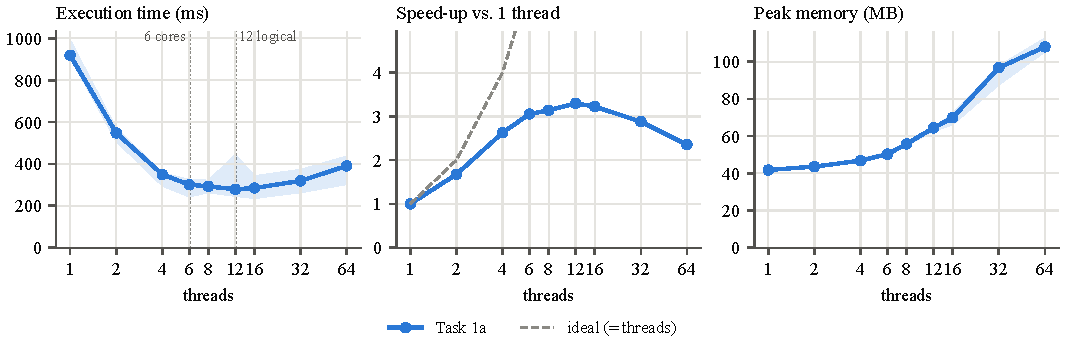
\includegraphics[width=\textwidth]{figures/task1a.pdf}
\caption{Task 1a: time, speed-up and peak memory against the number of threads (median of 5 runs;
the band shows the fastest and slowest run; dotted lines: 6 physical cores, 12 logical processors)}
\label{fig:1a}
\end{figure}

\begin{table}[H]
\centering\small
\begin{tabular}{rrrrr}
\toprule
Threads & Median time (ms) & Min--max (ms) & Speed-up & Peak memory (MB) \\
\midrule
1 & 919 & 908--996 & 1.00 & 42 \\
2 & 548 & 507--572 & 1.68 & 44 \\
4 & 350 & 294--359 & 2.63 & 47 \\
6 & 301 & 242--326 & 3.05 & 50 \\
8 & 293 & 262--323 & 3.14 & 56 \\
12 & 279 & 245--446 & 3.30 & 64 \\
16 & 285 & 235--344 & 3.22 & 70 \\
32 & 319 & 262--375 & 2.88 & 97 \\
64 & 391 & 301--438 & 2.35 & 108 \\
\bottomrule
\end{tabular}

\caption{Task 1a results}
\label{tab:1a}
\end{table}

\subsection{Task 1b: Three ways to count}

\textbf{Implementation} (\texttt{Task1b.java}). The whole file is first loaded into an
\texttt{int[]} of 50\,000\,000 elements (not measured). The array is divided into equal
contiguous parts, one per thread, and the program is run with
\texttt{--mode unsync|lock|local}. By default it uses as many threads as there are logical
processors, \texttt{Runtime.availableProcessors()}~=~12 on my laptop. The three versions differ
only in where a thread adds one to a counter:

\begin{lstlisting}
// 1: shared counters (plain fields of one shared object), no synchronisation
if (v < 0) shared.negative++; else if (v > 0) shared.positive++; else shared.zero++;

// 2: the same shared counters, every increment under a ReentrantLock
lock.lock();
try { if (v < 0) shared.negative++; else if (v > 0) shared.positive++; else shared.zero++; }
finally { lock.unlock(); }

// 3: local variables of the thread; written to its own Counts once, summed after join()
if (v < 0) negative++; else if (v > 0) positive++; else zero++;
\end{lstlisting}

Table~\ref{tab:1b-runs} shows every run with 12 threads (version~1 three times, as required, and
the other versions three times as well). Figure~\ref{fig:1b} and Table~\ref{tab:1b-threads}
show the three versions for all thread counts.

\begin{table}[H]
\centering\footnotesize\setlength{\tabcolsep}{4pt}
\begin{tabular}{lrrrrrrc}
\toprule
Version & Run & Time (ms) & Negative & Positive & Zero & Total & Correct \\
\midrule
1: shared, no sync & 1 & 330.1 & 3,369,126 & 3,360,083 & 25 & 6,729,234 & \textbf{no} \\
1: shared, no sync & 2 & 348.5 & 3,954,164 & 3,943,448 & 25 & 7,897,637 & \textbf{no} \\
1: shared, no sync & 3 & 331.2 & 3,402,233 & 3,391,194 & 25 & 6,793,452 & \textbf{no} \\
2: shared + lock & 1 & 794.6 & 25,001,107 & 24,998,868 & 25 & 50,000,000 & yes \\
2: shared + lock & 2 & 767.5 & 25,001,107 & 24,998,868 & 25 & 50,000,000 & yes \\
2: shared + lock & 3 & 736.1 & 25,001,107 & 24,998,868 & 25 & 50,000,000 & yes \\
3: per-thread counters & 1 & 72.7 & 25,001,107 & 24,998,868 & 25 & 50,000,000 & yes \\
3: per-thread counters & 2 & 83.3 & 25,001,107 & 24,998,868 & 25 & 50,000,000 & yes \\
3: per-thread counters & 3 & 74.8 & 25,001,107 & 24,998,868 & 25 & 50,000,000 & yes \\
\bottomrule
\end{tabular}

\caption{Task 1b with 12 threads (= logical processors): time and totals of every run. The correct
totals are 25\,001\,107 / 24\,998\,868 / 25 / 50\,000\,000}
\label{tab:1b-runs}
\end{table}

\begin{figure}[H]
\centering
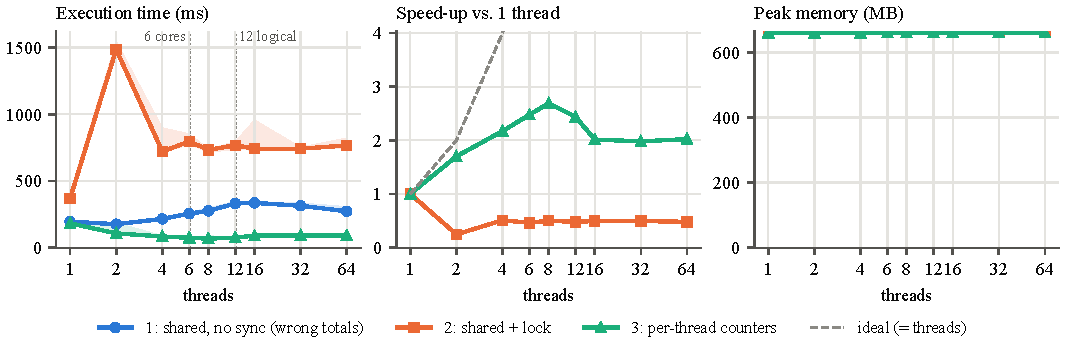
\includegraphics[width=\textwidth]{figures/task1b.pdf}
\caption{Task 1b: the three versions against the number of threads (median of 3 runs). Version 1
has no speed-up curve because its results are wrong. The peak-memory lines lie on top of each
other}
\label{fig:1b}
\end{figure}

\begin{table}[H]
\centering\small
\begin{tabular}{rrrrr}
\toprule
Threads & 1: no sync (ms) & 2: lock (ms) & 3: per-thread (ms) & 1: median total \\
\midrule
1 & 195 & 368 & 182 & 50.0M \\
2 & 176 & 1485 & 107 & 32.3M \\
4 & 215 & 721 & 84 & 21.3M \\
6 & 255 & 796 & 74 & 14.9M \\
8 & 276 & 733 & 68 & 12.2M \\
12 & 331 & 767 & 75 & 6.8M \\
16 & 336 & 741 & 90 & 7.2M \\
32 & 314 & 742 & 92 & 6.7M \\
64 & 273 & 765 & 90 & 6.6M \\
\bottomrule
\end{tabular}

\caption{Task 1b: median time of each version, and the median total counted by version 1 (it
should be 50.0M)}
\label{tab:1b-threads}
\end{table}

The peak memory is about 660\,MB for every version and thread count. It comes from loading the
array: the array grows by doubling while the file is read and is then trimmed to exactly
50\,000\,000 elements, so for a moment a 256\,MB and a 200\,MB array exist at the same time. The
counters themselves take a few bytes, so the memory does not depend on the version or the number
of threads.

\subsection{Task 1c: Producer and consumers}

\textbf{Implementation} (\texttt{Task1c.java}). The reader thread reads \texttt{numbers.txt}
line by line (\texttt{readLine()} of a \texttt{BufferedReader}) and collects the lines into \texttt{String[]} batches of
10\,000. It puts each batch into an \texttt{ArrayBlockingQueue} with capacity 100 batches, a
blocking queue from the Java library. \texttt{put()} blocks the reader while the queue is full,
and \texttt{take()} blocks a worker while the queue is empty. Java's \texttt{BlockingQueue} has no
\texttt{close()}, so the reader closes the queue another way. After the last batch it puts one
empty marker array (\texttt{END}) for every worker. The queue is FIFO, so a worker sees
\texttt{END} only after all real batches are taken, and then it stops. Every worker parses the
lines of its batches and counts into its own counters, which are added after \texttt{join()}. The
program also counts how often the reader found the queue full and how often a worker found it
empty, and the largest number of batches that were waiting in the queue.

\begin{figure}[H]
\centering
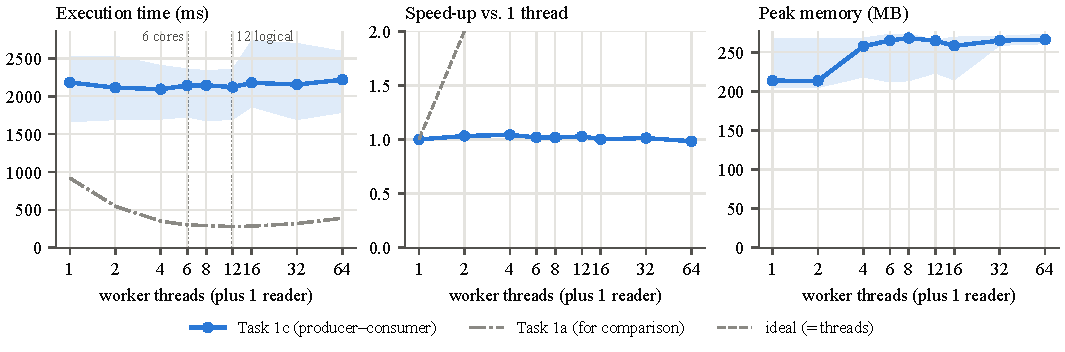
\includegraphics[width=\textwidth]{figures/task1c.pdf}
\caption{Task 1c: time, speed-up and peak memory against the number of workers (median of 5 runs;
the band shows the fastest and slowest run). The dash-dotted line is Task 1a}
\label{fig:1c}
\end{figure}

\begin{table}[H]
\centering\small
\begin{tabular}{rrrrr}
\toprule
Threads & Median time (ms) & Min--max (ms) & Speed-up & Peak memory (MB) \\
\midrule
1 & 2183 & 1664--2532 & 1.00 & 214 \\
2 & 2114 & 1691--2532 & 1.03 & 214 \\
4 & 2094 & 1699--2408 & 1.04 & 258 \\
6 & 2143 & 1727--2362 & 1.02 & 265 \\
8 & 2146 & 1678--2340 & 1.02 & 268 \\
12 & 2122 & 1694--2357 & 1.03 & 265 \\
16 & 2179 & 1863--2736 & 1.00 & 258 \\
32 & 2155 & 1693--2698 & 1.01 & 265 \\
64 & 2220 & 1788--2594 & 0.98 & 266 \\
\bottomrule
\end{tabular}

\caption{Task 1c results}
\label{tab:1c}
\end{table}

\begin{table}[H]
\centering\small
\begin{tabular}{rrrr}
\toprule
Workers & Worker waits (empty queue) & Reader waits (full queue) & Max batches in queue \\
\midrule
1 & 4975 & 0 & 48 \\
2 & 4999 & 0 & 6 \\
4 & 5001 & 0 & 6 \\
6 & 5003 & 0 & 4 \\
8 & 5006 & 0 & 5 \\
12 & 5011 & 0 & 1 \\
16 & 5012 & 0 & 2 \\
32 & 5029 & 0 & 2 \\
64 & 5061 & 0 & 5 \\
\bottomrule
\end{tabular}

\caption{Task 1c: how the queue was used (the file gives 5\,000 batches; waits are medians of 5 runs,
the queue length is the largest over the runs)}
\label{tab:1c-waits}
\end{table}

To answer question 6 by measurement and not only in words, I also ran Task 1c with batches of a
single line (\texttt{--batch 1}) and with a queue without a size limit (\texttt{--capacity 0}, which
uses a \texttt{LinkedBlockingQueue}), with 1, 4 and 12 workers (Table~\ref{tab:1c-var}, one run each;
the rows with batch 10\,000 and limit 100 are the medians from Table~\ref{tab:1c}).

\begin{table}[H]
\centering\footnotesize\setlength{\tabcolsep}{4pt}
\begin{tabular}{rrrrrrr}
\toprule
Batch (lines) & Queue limit & Workers & Time (ms) & Peak memory (MB) & Max batches in queue & Worker waits \\
\midrule
10,000 & 100 & 1 & 2183 & 214 & 48 & 4975 \\
1 & 100 & 1 & 13377 & 207 & 100 & 1428281 \\
10,000 & no limit & 1 & 2191 & 358 & 65 & 4475 \\
10,000 & 100 & 4 & 2094 & 258 & 6 & 5001 \\
1 & 100 & 4 & 19320 & 205 & 100 & 963760 \\
10,000 & no limit & 4 & 2143 & 258 & 1 & 5003 \\
10,000 & 100 & 12 & 2122 & 265 & 1 & 5011 \\
1 & 100 & 12 & 42159 & 205 & 100 & 932549 \\
10,000 & no limit & 12 & 2094 & 269 & 2 & 5011 \\
\bottomrule
\end{tabular}

\caption{Task 1c with other batch sizes and queue limits}
\label{tab:1c-var}
\end{table}

\subsection{Answers to the questions of Task 1}

\q{1. At which number of threads does the speed-up stop growing? Relate it to your physical cores
and logical processors.}
The speed-up grows fast up to 6 threads, my 6 physical cores (3.05$\times$), then only a little up
to 12, my 12 logical processors (3.30$\times$, the best). Two logical processors of one core share
its execution units, so the second one adds only 8\,\%. Above 12 the time grows again.

\q{2. Why do 32 and 64 threads not help? Are they slower, and why?}
They are slower: 319\,ms and 391\,ms against 279\,ms with 12 threads. Only 12 threads can run at
the same time, so the operating system has to switch between the others, and every switch, thread
start and extra read buffer only adds time.

\q{3. Does the peak memory depend on the number of threads? Why?}
A little in Task 1a: 42\,MB with 1 thread and 108\,MB with 64, about 1\,MB per thread, because every
thread has its own 1\,MiB read buffer and stack. In Task 1b (about 660\,MB, the loaded array) and
Task 1c (214--268\,MB, the queue and the strings) it does not depend on the threads.

\q{4. Rank the three versions of Task 1b by time. Which of them are correct? Explain each result.}
With 12 threads: per-thread counters about 75\,ms, no synchronisation about 330\,ms, lock about
770\,ms. Only the lock and the per-thread versions are correct.
\begin{itemize}
\item \emph{No synchronisation}: wrong, 6.7--7.9 million instead of 50 million. \texttt{counter++}
is read, add, write; two threads read the same value and one increment is lost.
\item \emph{Lock}: correct, but only one thread at a time can count, so it is slower than one
thread alone (368\,ms).
\item \emph{Per-thread counters}: correct and fastest, because the threads share nothing while
counting and the results are added once after \texttt{join()}.
\end{itemize}

\q{5. Compare Task 1c with Task 1a. Which one is faster, and why? At which number of workers
does Task 1c stop getting faster?}
Task 1a is faster: 279\,ms against about 2\,100\,ms. In Task 1c only one reader reads the file
and creates the strings, and the workers wait for it (they found the queue empty for almost every
batch). So Task 1c does not get faster after 1 worker.

\q{6. What would happen with batches of a single line? And with a queue that has no size limit?}
With batches of one line every line needs its own queue operation and lock, so it was 6--20 times
slower (13\,s with 1 worker, 42\,s with 12). A queue with no limit gave the same time here, because
the reader is the slow one; but if the workers were slower, the whole file could pile up in memory
(about 2.5\,GB). The limit of 100 batches makes the reader wait and keeps the memory small.

\section{Conclusion}

On my laptop (6 cores, 12 logical processors) all the work I measured, counting 50 million
numbers, was \textbf{CPU-bound}. I tell this by two checks: the time falls when threads are added
(as long as there are free cores), and the time is close to the time of the pure computation, with
no part spent waiting for a device.
\begin{itemize}
\item \emph{Task 1a}: the time fell from 919\,ms on 1 thread to 301\,ms at 6 threads and 279\,ms at
12. If the work were waiting for the disk, more threads would not have made it three times faster.
Beyond the 12 logical processors it got worse, because there was no more processor to give.
\item \emph{Task 1b}: the data is already in memory, so there is no I/O at all. The per-thread
version went from 182\,ms on 1 thread to 68\,ms at 8 threads.
\item \emph{Task 1c} is limited by the processor too, but by only \emph{one} core. The single
reader that reads the lines and creates the strings is the bottleneck: the workers find the queue
empty for almost every batch, and 1 to 64 workers all take about 2.1\,s.
\end{itemize}
None of these tasks was I/O-bound on my machine. The 369\,MB file fits easily in the 16\,GB of RAM,
so Windows keeps it in its file cache, and ``reading'' it is only copying memory. Work becomes
I/O-bound when the data has to come from a device much slower than the processor, which these
tasks did not do.

Synchronisation has a price that depends on how often it happens. A lock taken for every number
made Task 1b ten times slower than per-thread counters (about 770\,ms vs.\ 75\,ms) and never faster
than one thread. Batches of one line made Task 1c 6--20 times slower than batches of 10\,000. Shared
counters without synchronisation were both wrong (84--87\,\% of the increments lost) and over
4 times slower than per-thread counters (about 330\,ms). The fastest correct design was to share
nothing while working and combine the results once at the end.


\end{document}
